%
% instructions for "compiling":
%   latex main (first pass, also generates .aux file for bibtex)
%   bibtex main (generates .bbl file with bibliography)
%   latex main (second pass, incorporates bibliography)
%   latex main (do this if you still get messages about labels
%      having changed or missing references)
% to generate/view/print postscript:
%   dvips -o main.ps main 
%   gv main.ps (to view)
%   lpr main.ps (to print, or print from "gv")
% to generate/view/print PDF:
%   dvips -Pcmz -Ppdf -j0 -G0 -o main.ps main
%   ps2pdf main.ps main.pdf
%   acroread main.pdf (to view/print)
%   
\documentclass[11pt]{report}
\usepackage{amsmath}
\usepackage{algorithm}
\usepackage[noend]{algpseudocode}
\makeatletter
\def\BState{\State\hskip-\ALG@thistlm}
\makeatother

\usepackage{graphicx}
\graphicspath{ {images/} }
% miscellaneous packages
% FIX THIS -- can add to or change, but these are useful
%
% uncomment the following if your input includes characters other than
% 7-bit ASCII (e.g., accented characters)
%\usepackage[utf8]{inputenc}
%
\usepackage{amsmath}
\usepackage{graphicx}
\usepackage{moreverb}
\usepackage{url}

% double spacing
\usepackage{setspace}
\doublespacing

% hyphenation
\usepackage[english]{babel}
\selectlanguage{english}

% allow more figures on a page
\setcounter{topnumber}{10}
\setcounter{bottomnumber}{10}
\setcounter{totalnumber}{10}
\setcounter{dbltopnumber}{10}
\def\topfraction{1.0}
\def\bottomfraction{1.0}
\def\textfraction{0.0}
\def\dbltopfraction{1.0}

% margins
%\usepackage[letterpaper,top=2.0in,bottom=1.5in,left=1.5in,right=1.0in]
%	{geometry}
\usepackage[top=2.0in,bottom=1.5in,left=1.5in,right=1.0in]{geometry}

% set up to put page numbers in header
\usepackage{fancyhdr}
\pagestyle{fancy}
\lhead{}
\chead{}
\rhead{\rm\thepage}
\lfoot{}
\cfoot{}
\rfoot{}
\renewcommand{\headrulewidth}{0pt}
\renewcommand{\footrulewidth}{0pt}

% author, title, and date
% FIX THIS
\newcommand{\theAuthor}{Your Name Here}
% FIX THIS -- but be sure to leave in \par if title might exceed
%   one line -- otherwise space between lines will be wrong
\newcommand{\theTitle}{Your Title Goes Here
	(It Can Be Really Really Really Really Long)\par}
% FIX THIS
\newcommand{\theDate}{April 1, 2005}

\newlength{\WidthOfX}
% do not set here -- set just before use so we get the right font size
%\settowidth{\WidthOfX}{X} 
\newenvironment{TitlePageList}
{\begin{list}{}{%
  \setlength\leftmargin{0pt}%
  \setlength\labelwidth{10pt}%
  \setlength\itemindent{0pt}%
  \let \makelabel\descriptionlabel%
}}
{\end{list}}

% FIX THIS -- can put additional macro definitions here

%----------------------------------------------------------------------

\begin{document}

\pagenumbering{gobble}

%
% spacing could probably be improved
%

\begin{center}

\bigskip

\begin{Large}
\textbf{\theTitle}
\end{Large}

\bigskip

\begin{large}
\theAuthor
\end{large}

\bigskip
\bigskip

\textbf{Abstract}

\end{center}

\noindent
% FIX THIS --- your abstract goes here.
A nice abstract goes here.



\clearpage
%
% spacing could probably be improved
%
\begin{center}

\bigskip

\begin{Large}
\textbf{Acknowledgments}
\end{Large}

\bigskip

\end{center}

%FIX THIS --- thank your advisor, etc., here.
Some acknowledgments go here.



\clearpage
\begin{singlespace}

\begin{center}

\textbf{\theTitle} 

\vspace*{\baselineskip}

\theAuthor 

\vspace*{\baselineskip}

A departmental senior thesis submitted to the \\
Department of Computer Science at Trinity University \\
in partial fulfillment of the requirements for graduation \\
with departmental honors. 

\vspace*{\baselineskip}

\theDate

\vfill

$\overline{\mbox{\rule{0in}{0.16in}Thesis Advisor~~~~~~~~~~~~~~~~~~~~~~~~~~}}$ 
\hfill
$\overline{\mbox{\rule{0in}{0.16in}Department Chair~~~~~~~~~~~~~~~~~~~~~~~~}}$ 

\vspace*{2\baselineskip}

$\overline{\mbox{\rule{0in}{0.16in}
~~~~~~~~Associate Vice President~~~~~~~~
}}$ \\
for \\
Academic Affairs

\end{center}

\vfill

\begin{small}

\settowidth{\WidthOfX}{X}

% FIX THIS comment/uncomment \item lines so correct box is checked
\noindent
Student Copyright Declaration: the author has selected the following
copyright provision:

\begin{TitlePageList}
%\item{[X]}
\item{[\hspace*{\WidthOfX}]}
This thesis is licensed under the
Creative Commons Attribution-NonCommercial-NoDerivs License, which
allows some noncommercial copying and distribution of the thesis,
given proper attribution.  To view a copy of this license, visit
\url{http://creativecommons.org/licenses/} or send a letter to Creative
Commons, 559 Nathan Abbott Way, Stanford, California 94305, USA.

%\item{[X]}
\item{[\hspace*{\WidthOfX}]}
This thesis is protected under the provisions of U.S. Code Title 17.
Any copying of this work other than ``fair use'' (17 USC 107)
is prohibited without the copyright holder's permission.

%\item{[X]}
\item{[\hspace*{\WidthOfX}]}
Other:

\end{TitlePageList}

\vspace*{2\baselineskip}

\noindent
% FIX THIS comment/uncomment \item lines so correct box is checked
Distribution options for digital thesis:

\begin{TitlePageList}

\item{[X]}
%\item{[\hspace*{\WidthOfX}]}
Open Access (full-text discoverable via search engines)

%\item{[X]}
\item{[\hspace*{\WidthOfX}]}
Restricted to campus viewing only (allow access only on the Trinity
University campus via \url{digitalcommons.trinity.edu})

\end{TitlePageList}

\end{small}

\end{singlespace}


\clearpage
%
% spacing could probably be improved
%

\begin{center}

\vfill

\begin{Huge}
\textbf{\theTitle}
\end{Huge}

\bigskip \bigskip \bigskip

\begin{huge}
\theAuthor
\end{huge}

\vfill

\end{center}


\tableofcontents
\listoftables
\listoffigures

\clearpage
\pagenumbering{arabic}

% FIX THIS -- one file per chapter is good but not required
%
% FIX THIS -- remove/change, just some examples of things
%
\chapter{Example chapter}

Example chapter, with apologies to Alex Kolliopoulos,
from whose thesis the examples of math and tables were
borrowed.

\section{Examples of figures and tables}
\label{section:example-figtbl}

This section contains some words, plus
Figure~\ref{fig:xor} and 
Table~\ref{table:treepurpose}.

words, words, words, words,
words, words, words, words,
words, words, words, words,
words, words, words, words,
words, words, words, words,
words, words, words, words,
words, words, words, words,
words, words, words, words,

\begin{figure}[hbtp]
\begin{center}
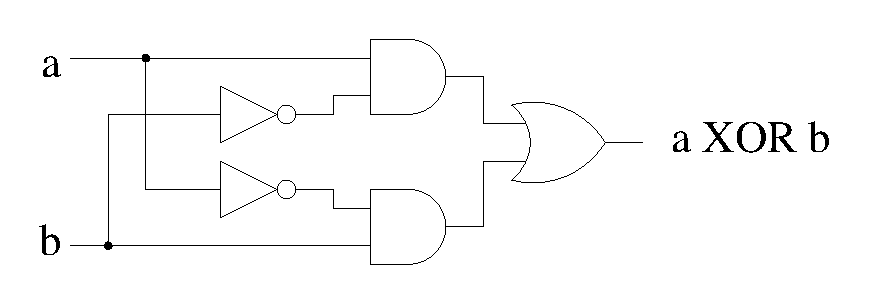
\includegraphics[width=0.5\textwidth]{xor}
\end{center}
\caption{An example figure.}
\label{fig:xor}
\end{figure}

words, words, words, words,
words, words, words, words,
words, words, words, words,
words, words, words, words,
words, words, words, words,
words, words, words, words,
words, words, words, words,
words, words, words, words,

\begin{table}[hbtp]
\begin{tabular}{|l|l|}
\hline 
\textbf{Trial 1} & Expanding a node to select a child\\
\hline
\textbf{Trial 3} & Selecting a node near the middle of a long, linear list\\
\hline
\textbf{Trial 4} & Selecting a node near the top of a long, linear list\\
\hline
\textbf{Trial 5} & Selecting a node near the bottom of a long, linear list\\
\hline
\textbf{Trial 6} & Scrolling and expanding folders in a large tree\\
\hline
\textbf{Trial 7} & Finding a node deep and near the bottom in a large tree\\
\hline
\textbf{Trial 8} & Finding a node near the top of a large tree\\
\hline
\end{tabular}
\caption{Purposes of each experimental trial.}
\label{table:treepurpose}
\end{table}
\section{Examples of math}
\label{section:example-math}

This section contains some math.
First, here's a set of equations.

\begin{eqnarray*}
y_p	&	=	&	\frac{y}{\sqrt{y^2+a^2}}, \\
y_p^2	&	=	&	\frac{y^2}{y^2+a^2}, \\
y_p^2	&	=	&	\frac{y^2+a^2-a^2}{y^2+a^2}, \\
y_p^2	&	=	&	1-\frac{a^2}{y^2+a^2}, \\
y_p^2-1	&	=	&	-\frac{a^2}{y^2+a^2}, \\
1-y_p^2	&	=	&	\frac{a^2}{y^2+a^2}.
\end{eqnarray*}

words, words, words, words,
words, words, words, words,
words, words, words, words,
words, words, words, words,
words, words, words, words,
words, words, words, words,
words, words, words, words,
words, words, words, words,

Now here's a numbered equation.

\begin{equation}
0 = 0 \label{eqn:example}
\end{equation}

\section{Examples of references}

% the "~" makes a no-line-breaks space
Section~\ref{section:example-figtbl} contains 
Figure~\ref{fig:xor} and
Table~\ref{table:treepurpose}.
Section~\ref{section:example-math} contains
Equation~(\ref{eqn:example}).
The sample bibliography file contains references to
a book \cite{gof-book} and a Web site \cite{MPI2}, plus some
other things.
% put in bibliography even though not referenced
\nocite{Dijkstra80}
\nocite{plop03-paper}


%
% FIX THIS -- remove/change, just some examples of things
%


\chapter{Partially Observable Environments}

\section{Introduction}
%this is how an image should look
%\includegraphics{universe}
Until now, both the GTGR and GTGRD models have given the observer full knowledge of the adversary's state for the entirety of the game. In real-world environments, observers may not have perfect information regarding the states and actions of an adversary. 

To accommodate for scenarios with incomplete information for the adversary, we introduce a partially observable variant of the GTGR scenario. In partially observable scenarios, the rules of the game remain largely unchanged, except for addition of “shadow states." The observer can not discern the current state of the adversary, while the adversary occupies a shadow state. When the adversary enters an observable portion of the graph, the observer will become aware of the adversary's position once more.

\begin{figure}[h!]
\begin{center}

  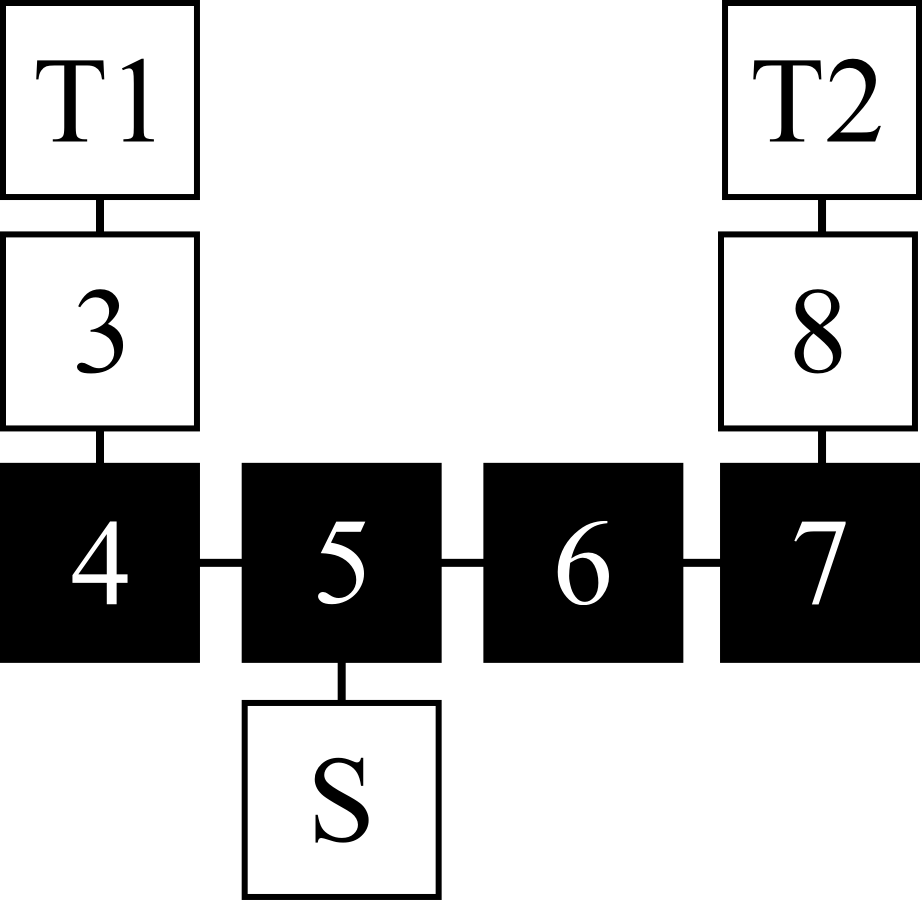
\includegraphics[scale=.15]{shadow1}
  \end{center}

  \caption{A partially observable graph.}
  \label{fig:shadow1}
\end{figure}

Figure~\ref{fig:shadow1} illustrates a partially observable environment. Visible states, in which the observer can see the adversary  white. Shadow states, in which the adversary is hidden from the observer, are black. The agent starts the game in state $S$. When the adversary moves to states $4$ ,$5$, $6$, or $7$, the observer is unable to determine their position until the adversary re-enters a visible portion of the graph.  
We will examine two solutions to the partially observable model, both of which involving linear programming. 

\section{The Whale Method}

The first method of solving partially observable environments, which we will call the "Whale Method," will utilize disjoint sets of shadow states. We call these sets of shadow states "shadow sets." We say that two shadow states belong to the same shadow set, if the adversary can travel between the two without entering an observable state.

\begin{figure}[h!]
\begin{center}

  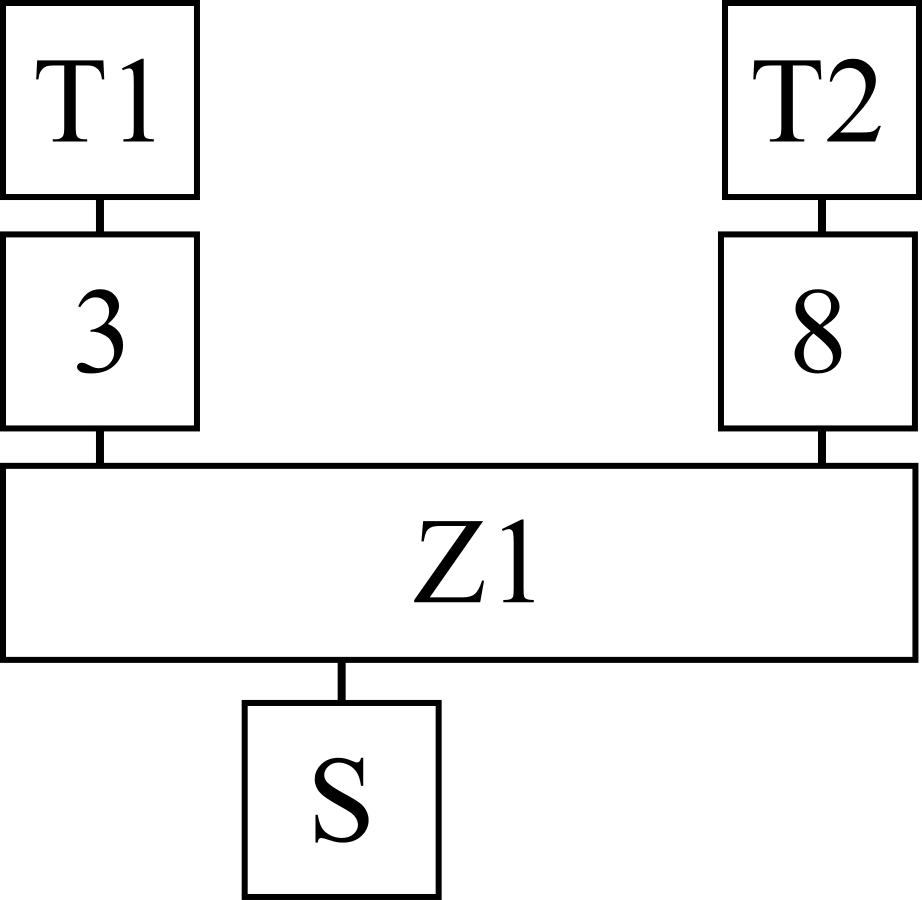
\includegraphics[scale=.15]{shadow2}
  \end{center}

  \caption{A partially observable graph with two shadow sets.}
  \label{fig:shadow2}
\end{figure}

The graph in Figure~\ref{fig:shadow2} has two disjoint shadow sets, one composed of states $2$ and $3$, the other composed of states $4$ and $5$. In using the Whale Method, the observer treats each shadow set a single state, which we will call a "whale state." We can identify the single shadow set in Figure~\ref{fig:shadow1}, composed of states $4$, $5$, $6$, and $7$. In using the Whale method, the observer treats each state in the shadow set as the same state. While the adversary may require several turns to travel among states $4$, $5$, $6$, and $7$, the adversary will act as if the has decided to remain stationary in the newly created state $W$ seen in Figure~\ref{fig:shadow3}

\begin{figure}[h!]
\begin{center}

  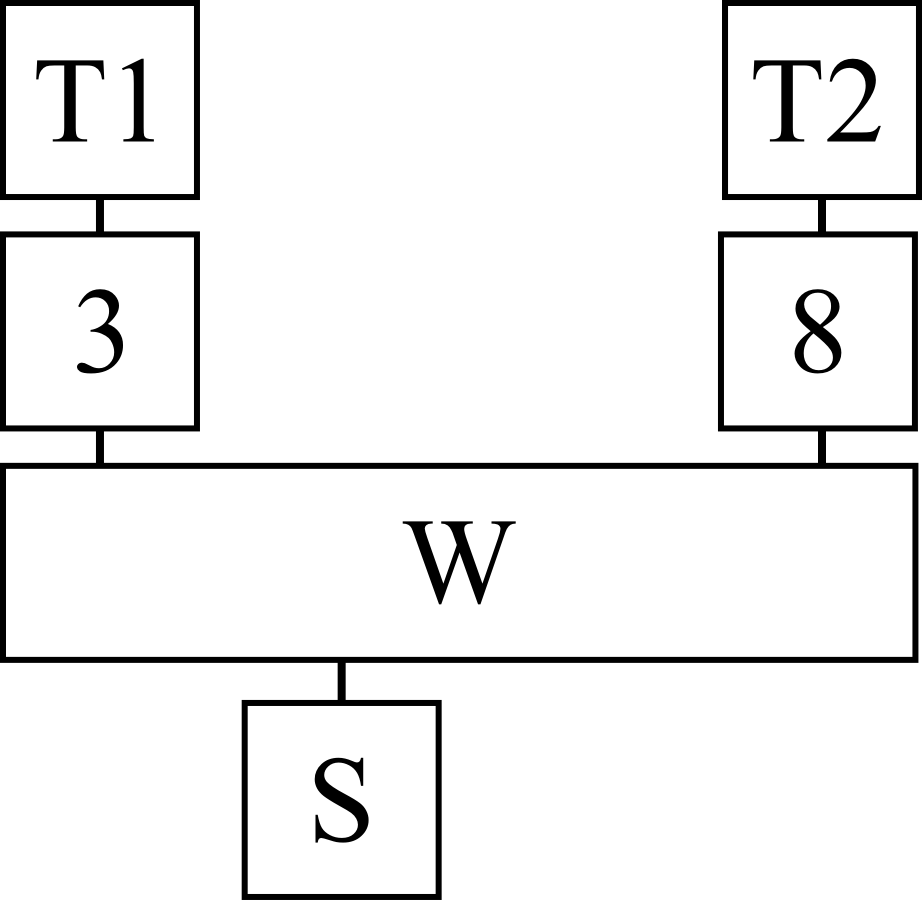
\includegraphics[scale=.15]{shadow3}
  \end{center}

  \caption{A partially observable graph with a single state in place of shadow states.}
  \label{fig:shadow3}
\end{figure}

We can add the following to the mixed integer program to accommodate for partially observable environments when using the Whale method.


\begin{equation}
V(\theta, s) \leq \sum_{i \in B} r(s, i, j, \theta)f_{i}(s) + V(\theta, j) \forall\theta\in B,\forall s \mid s\neq \theta, s\not\in H, \forall j\in\nu(s) \tag{3}
\end{equation}

\begin{equation}
V(\theta, s) \leq \sum_{i \in B} r(s, i, j, \theta)f_{w}(s) + V(\theta, j) \forall\theta\in B,\forall s \mid s\neq \theta, s\in H, \forall j\in\nu(s) \tag{3}
\end{equation}

\begin{equation}
\sum_{i} f_{i}(s) = 1\quad \forall s \tag{3}
\end{equation}

\begin{equation}
\sum_{w} f_{w}(s) = 1\quad \forall s \tag{3}
\end{equation}

\begin{equation}
f_{i}(s) \geq 0\quad \forall s,i\
\end{equation}

\begin{equation}
f_{w}(s) \geq 0\quad \forall s,w\
\end{equation}

We let $H$ denote the set of all shadow states, and $w$ denote the whale state the observer knows the adversary to be occupying. An observer action for any whale state $w$ is written as $f_{w}(s)$. These changes to the linear program require the observer to take the same action for each turn the adversary spends in a particular shadow set. The performance of the Whale method will be examined in a later section. 

\section{The Transmogrification Method}

When using the Whale method, the observer ignores some of the information available to them. The Whale method does not account for where the adversary entered a shadow set, or how long the adversary has remained hidden. The "Transmogrification Method" takes both of these pieces of information into account, by generating a fully observable environment from a partially observable environment. To do this, the observer must make some basic assumptions about the adversary's strategy. The following lemmas and corollary assume the agent is playing optimally against the observer's stationary strategy. 

\textbf{Lemma 2.} \textit{If the adversary's target does not lie within a shadow set, the adversary will eventually exit the shadow set.}

\textit{Proof (Sketch).} As mentioned previously, the game could theoretically go on forever. But because of the potential per-timestep cost of $d$ and the observer's predictions, any sufficiently long path for
the adversary would be dominated by the strategy of taking the shortest path to their target $\theta$. If the adversary never leaves the set of shadow states, then the game will go on forever. Thus, the adversary will eventually leave a shadow set. 

\textbf{Corollary 2.} \textit{An optimal agent occupying a state in a shadow set will take a shortest path to the exit state of their choosing.} 

\textit{Proof (Sketch).} We established that an optimal adversary in a shadow set must exit that shadow set. Each unnecessary turn the adversary spends in a shadow state invites the observer to guess their intended target. Thus, it is in the observer's interest to reach their chosen exit as quickly as possible.

With Corollary 2, the observer can generate a new graph to play on.

\begin{figure}[h!]
\begin{center}

  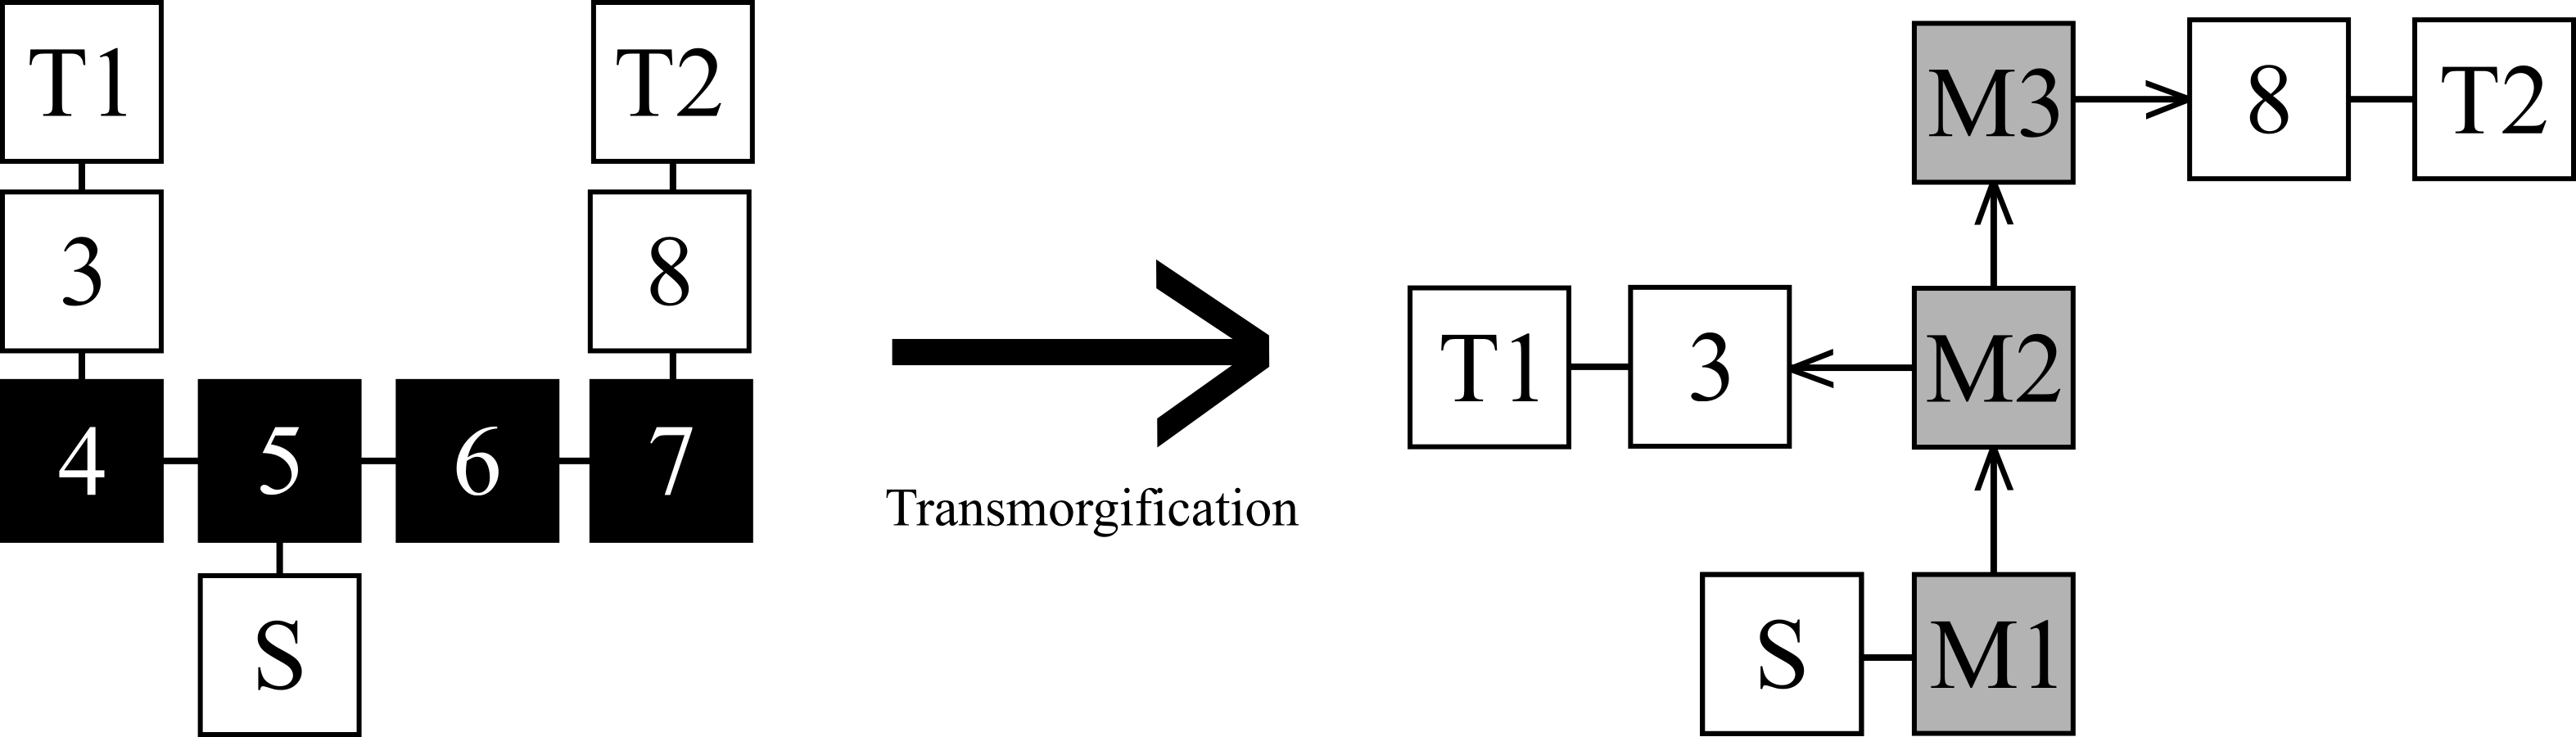
\includegraphics[scale=.15]{shadow4}
  \end{center}

  \caption{The partially observable environment from Figure~\ref{fig:shadow1} (left) transmogrified into an, fully observable graph.}
  
  \label{fig:shadow4}
\end{figure}

Figure~\ref{fig:shadow4} illustrates a transmogrified version of the graph from Figure ~\ref{fig:shadow1}. The grey nodes in the transmogrified graph are introduced to represent the number of turns the adversary has remained hidden from the observer. For instance, if the adversary has been hidden for two turns, then the observer would see the adversary as occupying state $M2$ in the transmogrified graph. Take note that the transmogrified graph now includes directed edges, because we are (hopefully) not dealing with a time traveling agent. To generate these graphs, we examine each shadow set. For each shadow set, we examine each "entrance state" connected by an edge to the shadow state. We then compute the shortest path between every two entrance states for that shadow state. By Corollary 2, we assume the length of the longest shortest path will be the maximum number of turns an optimal agent will spend within the shadow set. We then create create the same number of memory nodes with directed edges from one to the next (see states $M1, M2, M3$ from state $S$ in Figure ~\ref{fig:shadow4}). Then we create an edge from each entrance state, to the memory state corresponding to the length of the shortest path between the entrance state, and the original entrance state from which we spawned the memory states. For example, because a adversary would have to two shadow states on their journey from state $S$ to state $3$ in Figure ~\ref{fig:shadow1}, we connect state $M2$ to state $3$ in Figure ~\ref{fig:shadow4}. Note, that the post transmogrification graph in Figure ~\ref{fig:shadow4} is actually incomplete, because memory states have only been spawned from the entrance state $S$ and not from entrance states $3$ or $8$. Because an optimal agent has no reason to backtrack in this particular scenario, the memory nodes for $3$ and $8$ were omitted to keep the graph simple.

\begin{figure}[h!]
\begin{center}

  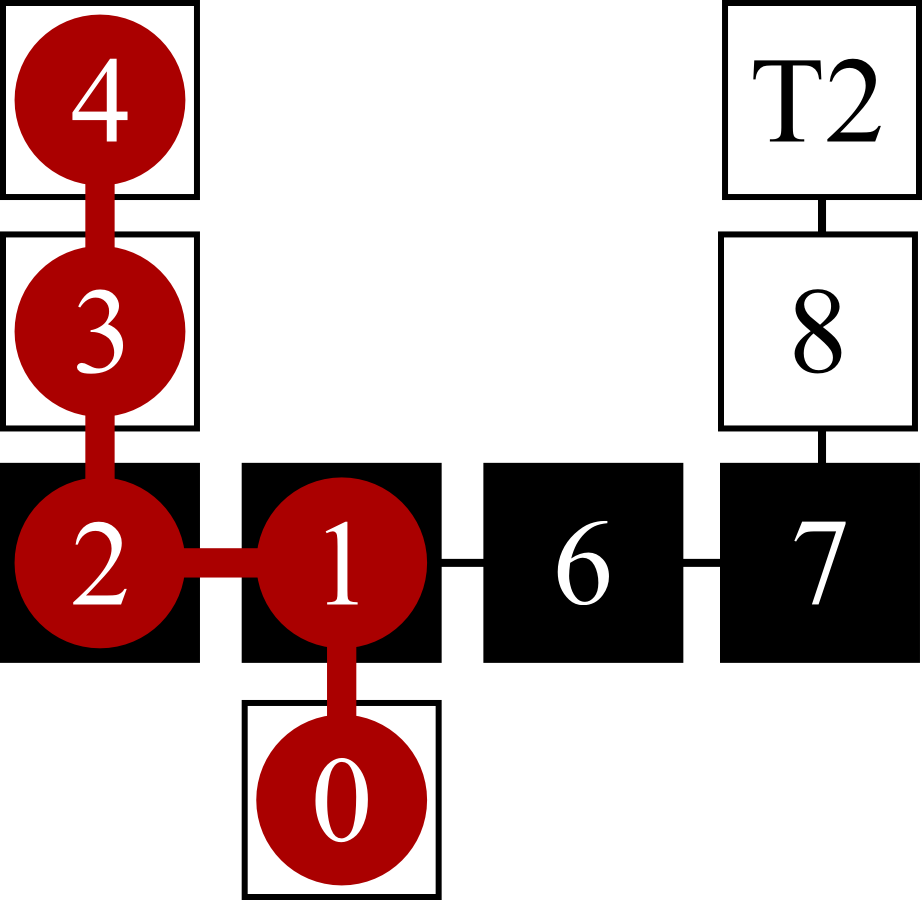
\includegraphics[scale=.15]{shadow5}
  \end{center}

  \caption{The adversary's path to target $T1$.}
  
  \label{fig:shadow5}
\end{figure}

Next, let us examine how a game might play out from the adversary's perspective.   Using the environment from Figure ~\ref{fig:shadow1}, let us assume the adversary was assigned target $T1$. Because the graph is rather limiting, the adversary takes the shortest path from starting state $S$ to the target $T1$. Figure ~\ref{fig:shadow5} illustrates the adversary's journey, each turn market with a red circle. Note that on turns $1$ and $2$, the observer would lose sight of the attacker until turn $3$. Now, let us examine what the same scenario would look like from the observer's prospective, when using the transmogrification method. 

\begin{figure}[h!]
\begin{center}

  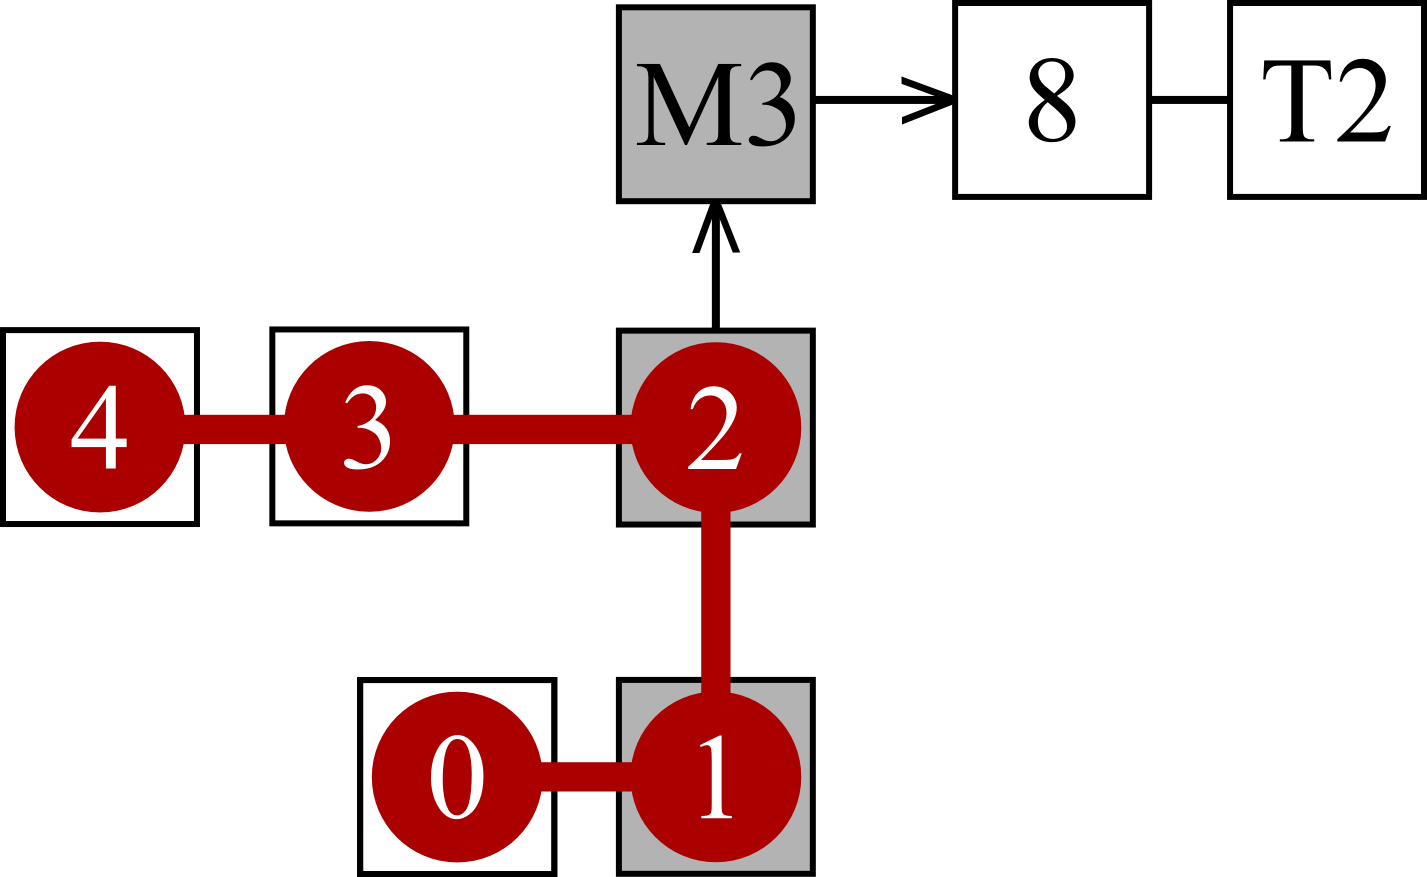
\includegraphics[scale=.15]{shadow6}
  \end{center}

  \caption{The adversary's path to $T1$ from the observer's perspective.}
  
  \label{fig:shadow6}
\end{figure}

Because the adversary takes two turns within the shadow set, the observer sees the adversary as moving from state $M1$ to state $M2$, before exiting the shadow set on turn 3. 

%explain code sample down below

\section{Experiments}

As with previous experiments, all tests were run on  a machine using OSX Yosemite version 10.10.5, with 16 GB of ram and a 2.3 GHz Intel Core i7 processor. First, we will use the simple example from Figure ~\ref{fig:shadow1} to compare the performance of the Whale, and Transmogrification methods. Additionally, we will compare the performance against a best case solution, in which we turn all shadow states into standard states. The best case solutions measures how the observer would perform if their strategy effectively negated the shadow states. Graphs were displayed using the Python NetworkX library. Arrowheads on directed edges were added manually for clarity. The starting state is displayed in green, target states are displayed in red, shadow states are displayed in purple, and default states are displayed in cyan.

\begin{figure}[h!]
\begin{center}

  \includegraphics[scale=.15]{test1}
  \end{center}

  \caption{A simple scenario using NetworkX.}
  
  \label{fig:test1}
\end{figure}

After transmogrifying the graph, the scenario becomes more complex, but allows the observer to play a fully observable game. There graph will no longer have any shadow states (purple). All states labeled with values greater than 1000 are nodes that have been added to represent turns hidden within the shadow set. Note that the graph in Figure ~\ref{fig:test2} will have more nodes than the previously seen illustration of the transmogrified graph in Figure ~\ref{fig:shadow4}, because we spawn memory states for every entry state, and not just the starting state. 

\begin{figure}[h!]
\begin{center}

  \includegraphics[scale=.15]{test2}
  \end{center}

  \caption{The transmogrified graph.}
  
  \label{fig:test2}
\end{figure}

For this game, the adversary is not penalized for timesteps taken. The reward for reaching the target is 0. The reward the observer receives for each correct guess was set to 1. The point value for each method at the end of the game equates to the number of correct guesses the observer can expect to make. At the start of the game, the adversary has a 75\% chance of being assigned target $1$, and a 25\% of being assigned target $2$.

\begin{table}[hbtp]
\begin{center}
\begin{tabular}{|l|l|}
\hline 
\textbf{No Shadow States} & 3.75 Correct Guesses\\
\hline
\textbf{Whale} & 3.25 Correct Guesses\\
\hline
\textbf{Transmogrification} & 3.50 Correct Guesses\\
\hline
\end{tabular}
\end{center}
\caption{Performance results from simple environment.}
\label{table:simpletable}
\end{table}

If a strategy were to effectively remove the shadow states from the board, the observer could expect to make 3.75 correct guesses over the course of the game. Thus, we could not expect the whale or transmogrification methods to perform any better. Using the whale methods, in which all shadow states a mushed together into one whale of a state, the observer can expect to make 3.25 correct guesses. While the transmogrification method does not allow the observer to effectively see through shadow states, the method still outperforms the whale method with a score of 3.50. Next, we will test these methods against each other in a more complex scenario.  

\begin{figure}[h!]
\begin{center}

  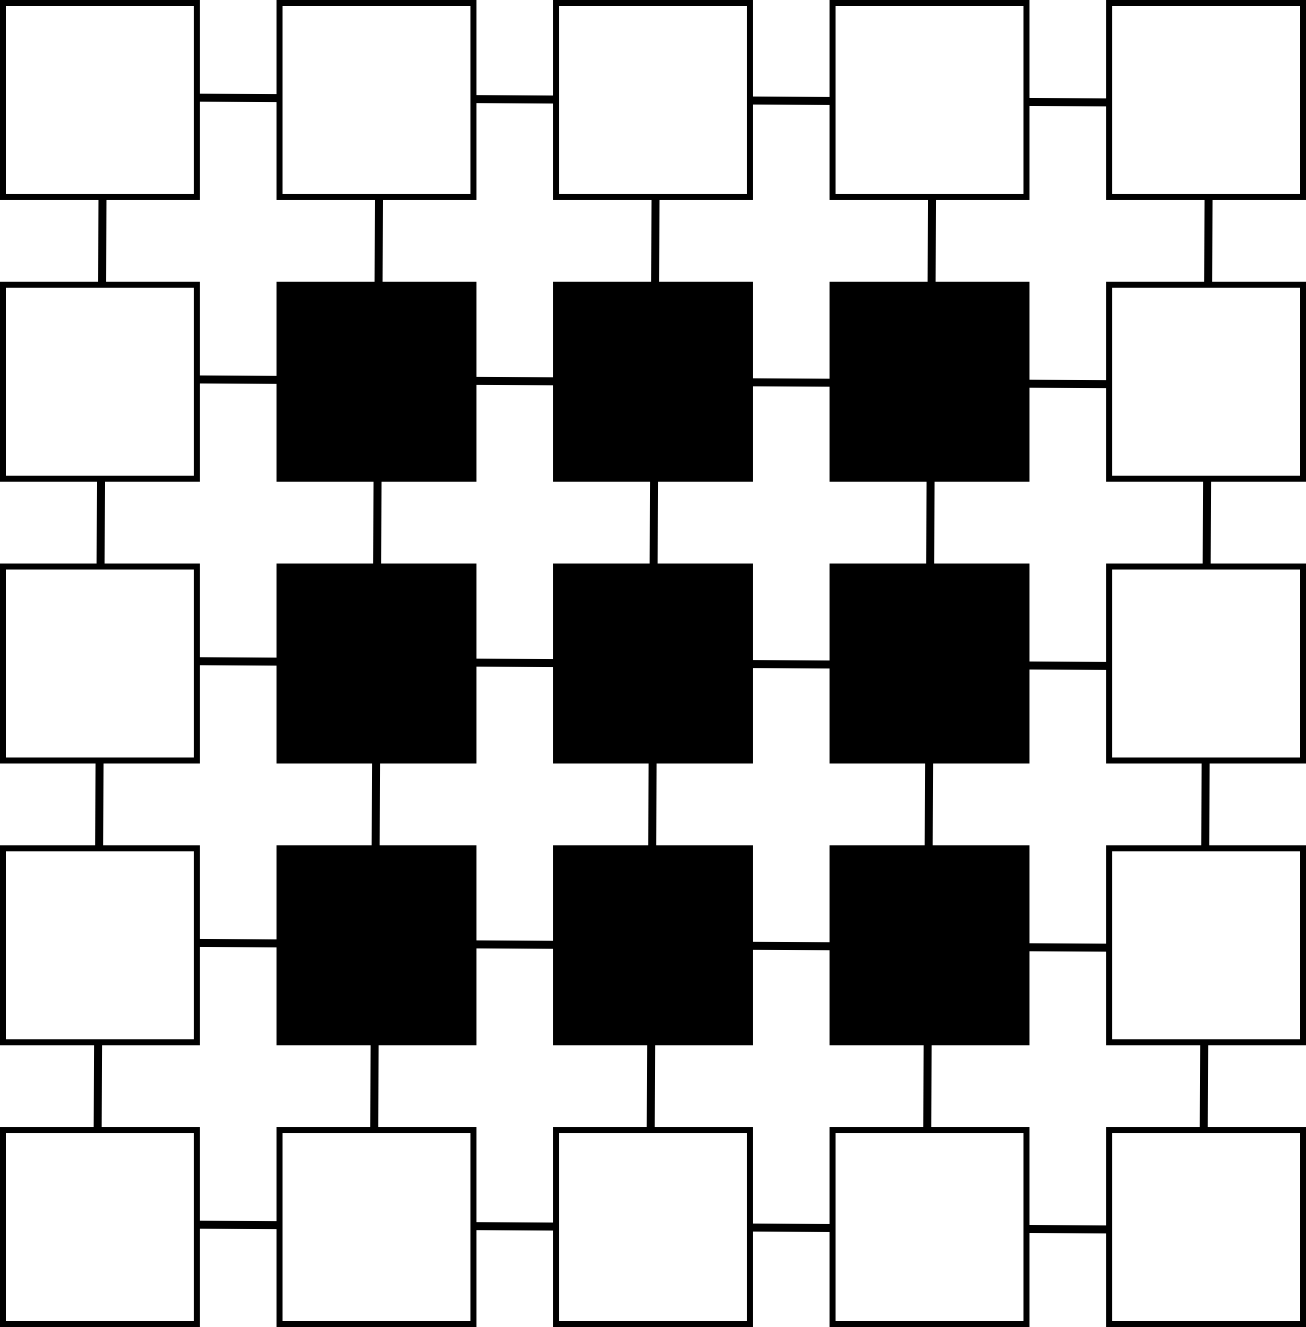
\includegraphics[scale=.15]{arena}
  \end{center}

  \caption{Complex testing environment.}
  
  \label{fig:arena}
\end{figure}

With the simple example out of the way, we move to a more complex environment which offers the adversary more freedom in approaching their target. For the next set of tests, we place the adversary starting state, and 3 potential targets on non-shadow states (marked in white) in Figure ~\ref{fig:arena}. We then create a random probability distribution, and solve the game with both methods. After ten-thousand iterations, the scores are averaged and compared. 

\begin{table}[hbtp]
\begin{center}
\begin{tabular}{|l|l|}
\hline 
\textbf{No Shadow States} & 2.65 Correct Guesses\\
\hline
\textbf{Whale} & 2.41 Correct Guesses\\
\hline
\textbf{Transmogrification} & 2.59 Correct Guesses\\
\hline
\end{tabular}
\end{center}
\caption{Average method performance in complex environment.}
\label{table:simpletable}
\end{table}

Though the transmogrification method does not yield what the observer could score without shadow states, it still outperforms the whale method.

\nocite{Dijkstra80}
\nocite{plop03-paper}


% FIX THIS -- refs.bib is the bibtex file
\bibliography{refs}
\bibliographystyle{plain}

\appendix
% FIX THIS
%
% FIX THIS -- remove/change, just an example of a simple way to
%   include a lot of code (hello.c here)  
%

\chapter{Example appendix}

Here is my code.

\begin{singlespacing} 
\begin{small}
\verbatimtabinput{hello.c}
\end{small}
\end{singlespacing}


\end{document}
